\chapter{Digital Video Broadcasting (DVB)}
There are many parts that are needed to provide Digital Video 
Broadcasting (DVB) with a secure way of transmitting streams of data 
without facing the risk of content getting stolen. The following parts 
will be treated in this thesis:

\begin{itemize}
\item Head-end - explained in section \ref{sec:HE}
\item CA system (CAS) - explained in section \ref{sec:CAS}
\item Common Interface - explained in section \ref{sec:CI}
\item Scrambler - explained in chapter \ref{ch:Scrambling}
\item Descrambler - the inverse of a scrambler.
\end{itemize}

The parts are connected according to figure \ref{fig:system}. The CAM is
explained in section \ref{sec:CAM}, the ECM and EMM signals are 
mentioned briefly in section \ref{sec:CAS} and the DVB-SimulCrypt is 
described in section \ref{sec:Simul}.

\begin{figure}[h!]
  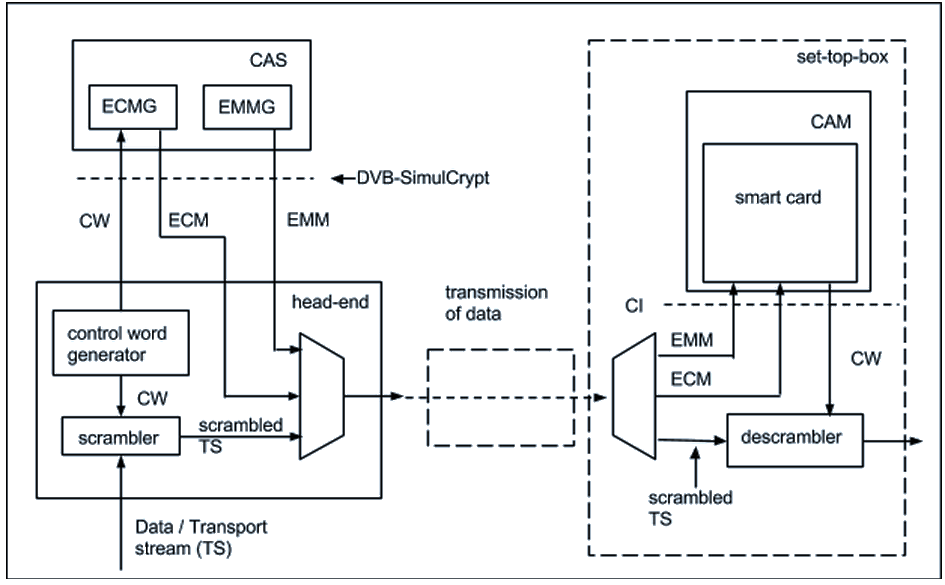
\includegraphics[width=\textwidth]{system}
  \caption{The DVB setup}
  \label{fig:system}
\end{figure}

\section{Head-end} \label{sec:HE}
The head-end is the part where the scrambler is located. Except for the 
scrambler, decoding and generation of program specific information takes
place in the head-end. After receiving data from content providers, it 
decodes, encrypts and encapsulates the data, before transmitting it.

\section{Control word} \label{sec:setup}
\emph{Transport Stream}s (TS), which contain data received from 
distributors, are scrambled using a key which is called a \emph{control 
word}. Control words are usually changed every 120th second, but might 
be changed more often. Some systems change the control word every 10th 
second. Finding out just one control word has very little effect on 
content theft, since it will only be usable for a few seconds before 
changed. Because of the high frequency in which the control words are 
changed, one means of security is provided. The control words are 
generated randomly to make sure that consecutive control words can not 
be derived from each other.

The control word is sent to a \emph{Conditional Access System} 
(CA system) where the control word is encrypted as an 
\emph{Entitlement Control Message} (ECM). The CA system also generates 
an \emph{Entitlement Management Message} (EMM) which tells the 
smart card what contents the user is allowed access to. This could for 
instance be whether the user has paid to view premium football games or 
not. The ECM and EMM are then sent back to the head-end where they are 
attached to the scrambled TS packet using a multiplexer. This package 
is sent to a receiver, which is usually a TV. The ECM, EMM and TS 
packet are separated when they arrive. The ECM and TS packet are sent 
through a \emph{Common Interface} (CI) to a \emph{Conditional Access 
Module} (CAM), where the ECM (previous control word) is decrypted using 
a decryption algorithm located on a smart card. The resulting control 
word is then used to descramble the TS packet. The TS packet is 
encrypted once more if the CI is a CI-Plus, otherwise it is sent in the 
clear back to the receiver where the data is processed before it is 
dispatched to the user. The CI and CI-Plus as well as the extra 
encryption are all discussed in section \ref{sec:CI}.

\section{Conditional Access System} \label{sec:CAS}
To make sure that users fulfills a set of criteria, before being 
allowed to access content, \emph{Conditional Access} (CA) is used. 
Conditional Access is provided, based on information about the user, 
in a system seperate from the head-end. Content is first scrambled, and 
decoded in a head-end. The control word, used to scramble the data, is 
sent to the Conditional Access system (CAS) where it is encoded. The CA 
system consists of an EMM-generator (EMMG) and an ECM-generator (ECMG) 
among others. An ECM-generator encrypts the control word. The 
algorithms used in the generators differ between CA systems and is kept 
very secret, to make sure that the control word can not be stolen 
during transmission.

The ECM is generated using the control word, while the EMM is generated 
based on subscription- and payment information related to the user. The 
EMM can allow things, stretching from allowing a user to view a video 
for a few hours, to access a certain channel for an extended period of 
time. A TV will not display any channels without receiving an EMM 
allowing it to.
%\Warning[Source]{You need to find more sources than just Patrik}

An example is that a user needs to pay for TV-services to be able 
to access content. The CA system generates an EMM which tells 
the smart card whether the user is allowed to access the requested 
material or not. The content provider also generates an ECM based on 
the control word, which the smart card decrypts and passes to the 
descrambler, to decrypt the video stream. This is done if the EMM 
allows it.

\subsection{Standards}
Some of the CA systems currently in use are Viaccess, Conax, Irdeto, 
NDS, Strong and NagraVision. The CA systems are paired with 
\emph{Conditional Access Module}s (CAM), which are located in the 
receiver. What CAS / CAM pair depends on the content provider. For 
instance, NDS is used by Viasat, Conax is used by Com Hem, Viaccess 
is used by Boxer and Strong is used by Canal Digital. 

\begin{longtable}{| l | c | c |}
  \hline
  CA system & Used by & Supports CI+ \\ \hline
  
  Viaccess & Boxer, SVT & Yes \\ \hline
  Conax & Com Hem & Yes \\ \hline
  Strong & Canal Digital & Yes \\ \hline
\end{longtable}

\section{DVB-SimulCrypt} \label{sec:Simul}
The control words used during scrambling can be sent to several 
different CA systems at once (for reference, see section 
\ref{sec:CAS}), resulting in several ECMs. This is called 
DVB-SimulCrypt, which is widespread in Europe. DVB-SimulCrypt works as 
an interface between the head-end and the CA system. DVB-SimulCrypt 
encourages the use of several CA systems at once 
\citep{SimulCrypt:2008}. This is done by sending the same control word 
to many CA systems at the same time, and then allowing them to generate 
an ECM and EMM based on the control word. The multiplexer in the 
head-end then creates TS packets based on those, since the EMMs will 
determine whether the user is allowed access or not. A multiplexer is 
a basic logic circuit, which merges severals signals into a single 
signal.
%OERHÖRT CHANSAT DETTA JA OKEJ KOLLA ÖVER DET! Allt i detta stycke är chansat.

\section{Common Interface} \label{sec:CI}
The Common Interface is the interface between the CAM and the host 
(Digital TV receiver-decoder). There are currently two versions of 
common interfaces in use, which are the CI and the CI+. The difference 
between them is that the output from the CI is unencrypted, while the 
output from the CI+ is encrypted \citep{CI+:2011}. This means that a 
clear TS packet is sent between the CI and the host, that can be 
copied. The data sent between the CI+ and host can not be copied due 
to it being encrypted, and therefore provides more security for 
content providers \citep{CI:1997}.

\subsection{CI-Plus}
The CI-Plus realizes the possibility of yet another means of protecting 
content, which is called \emph{Content Control}. Content control is a 
way of encrypting the content inside of the CAM, connected to the 
CI-Plus Module. The key used for the content control encryption is 
paired with the Digital TV Receiver, where the TS packet is decrypted 
before being made available to users. The general idea can be viewed 
in Figure \ref{img:CIPlus}.

\begin{figure}[h!]
  \centering
  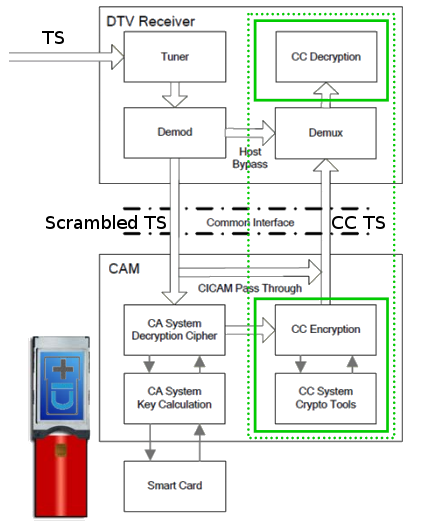
\includegraphics[width=0.5\textwidth]{CIPlus}
  \caption{CI-Plus interface. \citep[p. 10]{CI+:2011}}
  \label{img:CIPlus}
\end{figure}

CI-Plus encoding is often used to protect HD content, but not SD 
content. Since HD content is more high-profile, content distributors 
want to protect it more than the SD content. Protection of HD content 
requires scrambling using AES-128 in CBC-mode. 
\citep{CI+:2011, CI+:2011_2}

\section{Conditional Access Module}\label{sec:CAM}
CA modules (CAMs) are responsible of decoding the scrambled TS packet
received from the host. The CAM is inserted into a PCMCIA slot 
(Personal Computer Memory International Association) either into the TV 
or the set-top box. A set-top box is a box which you connect between 
the TV signal source and the TV. The set-top box is equipped with both 
a CI or CI-Plus, and a CAM. The CAM consists of a slot for a 
smart card and a descrambler. The smart card decodes the ECM and sends 
the control word back to the descrambler. The TS packet is then 
descrambled and the clear data is sent back to the host, from the CAM.
